\theoremstyle{definition}
\newtheorem{definition}{Definition}

\subsubsection{The Basic \queryfunc\ Algorithm}
\label{sec:collocation-algorithm}

We need to define function \queryfunc\ called
by the prefix tree algorithm (Listing~\ref{alg:prefix-tree}).
Its input consists of set $M_{a\alpha}$ representing all
{\em matchings} of prefix $a\alpha$ and set $M_{\alpha{}b}$ representing all
matchings of suffix $\alpha{}b$.  From this it must compute 
all matchings $M_{a\alpha{}b}$ of query pattern $a\alpha{}b$.

Recall from \textsection\ref{sec:baseline} that
a matching in the text for pattern 
$\alpha = w_1 X ... X w_{K_\alpha}$ is a $K_\alpha$-tuple 
$m_\alpha = (m_{\alpha,1}, ..., m_{\alpha,K_\alpha})$. 
The $k$th element $m_{\alpha,k}$ of $m_\alpha$ is the starting index
of a substring in $T$ matching subpattern $w_k$.  If two patterns
differ only by preceding or following nonterminal symbol $X$, then
their matchings in $T$ are identical.  More formally, 
if $\alpha = \beta{}X$ or $\alpha = X\beta$ then 
$M_\alpha = M_\beta$.  If $\alpha = X$
then $M_\alpha = ()$, the empty tuple.

For the discussion that follows, we will find it useful to 
define several formal properties of matchings.  First, we define an ordering.
For matchings $m_\alpha$ and $m_\alpha'$ of pattern $\alpha$,
$m_\alpha < m_\alpha'$ if and only if $\exists_{k \in \{1,...,K_\alpha\}} (m_{\alpha,k} < m'_{\alpha,k}$ and $\forall_{\ell \in \{1,...,k-1\}}  m_{\alpha,\ell} = m'_{\alpha,\ell})$.
Thus, a set of $K_\alpha$-tuples is ordered on the first index, 
then the second, and so on.

The {\em suffix matching} $s(m_{a\alpha})$ of 
matching $m_{a\alpha}$ is 
the embedded matching of suffix $\alpha$.
If $\alpha = X\beta$ and $m_{\alpha} = s(m_{a\alpha{}})$
then $K_{\alpha} = K_{a\alpha}-1$ and
$m_\alpha = (m_{a\alpha,2},...,m_{a\alpha,K_{a\alpha}})$.
If $\alpha = \beta{}c$ and $m_{\alpha} = s(m_{a\alpha{}})$
then $K_{\alpha,1} = K_{a\alpha,1}+1$, $m_{\alpha,1} = m_{a\alpha,1}+1$ and 
$\forall_{k \in \{2,...,K_{\alpha}\}} m_{\alpha,k} = m_{a\alpha,k}$.

The relationship between a matching and its suffix matching are shown in Figure~\ref{fig:matching-relationships}.

Analogously, the {\em prefix matching} $p(m_{\alpha{}b})$ of 
matching $m_{\alpha{}b}$ of pattern $\alpha{}b$ is 
the embedded matching of its prefix $\alpha$.
If $\alpha = \beta{}X$ and $m_{\alpha} = p(m_{\alpha{}b})$
then $K_{\alpha} = K_{\alpha{}b}-1$ and 
$m_\alpha = (m_{\alpha{}b,1},...,m_{\alpha{}b,K_{\alpha}})$.
If $\alpha = \beta{}c$ and $m_{\alpha} = p(m_{\alpha{}b})$
then $K_{\alpha} = K_{\alpha{}b}$ and $m_{\alpha} = m_{\alpha{}b}$.

\figpreamble
\begin{figure}
	\figfontsize{
	\begin{center}
		\begin{tikzpicture}
	\matrix (text) [inner sep=0pt,matrix of nodes,nodes={inner sep=3pt,draw,rectangle,anchor=center,minimum height=6.5mm}] {
		$\cdots$ & $a$ & $\longleftarrow X\longrightarrow$ & $\longleftarrow\beta\longrightarrow$ & $b$ & $\cdots$ \\
	};
	\draw[white,line width=4pt] (text.north east) -- (text.south east);
	\draw[white,line width=4pt] (text.north west) -- (text.south west);
	
	\node at (text-1-2.south west) [anchor=north west] {$i$};
	\node at (text-1-4.south west) [anchor=north west] {$j_1, \cdots, j_{m}$};
	
	\draw[snake=brace,raise snake=8mm,segment amplitude=1mm] (text-1-2.north west) -- (text-1-5.north east);
	\path (text-1-2.north west) -- (text-1-5.north east) coordinate [pos=0.5](midpoint);
	\node[anchor=south,above=8mm] at (midpoint) {$m_{a\alpha b} = (i, j_1, \cdots, j_{m})$};

	\draw[snake=brace,raise snake=1mm,segment amplitude=1mm] (text-1-3.north west) -- (text-1-5.north east);
	\path (text-1-3.north west) -- (text-1-5.north east) coordinate [pos=0.5] (midpoint);
	\node[anchor=south,above=1mm] at (midpoint) {$s(m_{a\alpha b}) = (j_1, \cdots, j_{m})$};

	\node [anchor=south,above=1.4cm] at (text.north west) {(1) $\alpha=X\beta$};

	% case 2
	\matrix (text) [inner sep=0pt,matrix of nodes,nodes={inner sep=3pt,draw,rectangle,anchor=center,minimum height=6.5mm},anchor=west,right=1.5cm] at (text.east) {
		$\cdots$ & $a$ & $c$ & $\longleftarrow\beta\longrightarrow$ & $b$ & $\cdots$ \\
	};
	\draw[white,line width=4pt] (text.north east) -- (text.south east);
	\draw[white,line width=4pt] (text.north west) -- (text.south west);

	\node at (text-1-2.south west) [anchor=north west] {$i$};
	\node at (text-1-3.south west) [anchor=north west] {$i+1, j_1, \cdots, j_{m}$};
	
	\draw[snake=brace,raise snake=8mm,segment amplitude=1mm] (text-1-2.north west) -- (text-1-5.north east);
	\path (text-1-2.north west) -- (text-1-5.north east) coordinate [pos=0.5](midpoint);
	\node[anchor=south,above=8mm] at (midpoint) {$m_{a\alpha b} = (i, j_1, \cdots, j_{m})$};

	\draw[snake=brace,raise snake=1mm,segment amplitude=1mm] (text-1-3.north west) -- (text-1-5.north east);
	\path (text-1-3.north west) -- (text-1-5.north east) coordinate [pos=0.5] (midpoint);
	\node[anchor=south,above=1mm] at (midpoint) {$s(m_{a\alpha b}) = (i+1, j_1, \cdots, j_{m})$};

	\node [above=1.4cm,anchor=south] at (text.north west) {(2) $\alpha = c\beta$};

\end{tikzpicture}
	\end{center}}
	\figpostamble
	\caption[Relationship between a matching $m{_{a\alpha{}b}}$ of pattern $a\alpha{}b$ and its suffix matching $s(m_{a\alpha{}b})$.]{Relationship between a matching $m{_{a\alpha{}b}}$ of pattern $a\alpha{}b$ and its suffix matching $s(m_{a\alpha{}b})$ for two cases, depending on whether the first symbol in $\alpha$ is a nonterminal or terminal.  Note that in both cases, there is only a single difference between the matchings.  In case (1), there is an additional index.  In case (2), the first index of each matching differs by exactly one.  The situation for prefix matchings is analogous.}
	\label{fig:matching-relationships}
\end{figure}

Note that $p(s(m_{a\alpha{}b})) = s(p(m_{a\alpha{}b}))$.
This gives a means to identify pairs $(m_{a\alpha}, m_{\alpha{}b})$
that imply a matching of $a\alpha{}b$.  Specifically, if 
$s(m_{a\alpha}) = p(m_{\alpha{}b})$, then we say that
$m_{a\alpha}$ and $m_{\alpha{}b}$ are {\em partners}
and we can {\em join} ($\bowtie$) them to form $m_{a\alpha{}b}$.
If $\alpha=\beta{}X$ and $m_{a\alpha{}b} = m_{a\alpha} \bowtie m_{\alpha{}b}$ 
then $K_{a\alpha{}b} = K_{a\alpha}+1$,
$\forall_{k \in \{1,...,K_{a\alpha}\}} m_{a\alpha{}b,k} = m_{a\alpha,k}$
and $m_{a\alpha{}b,K_{a\alpha{}b}} = m_{\alpha{}b,K_{\alpha{}b}}$.
Otherwise, if $\alpha=\beta{}c$ then $K_{a\alpha{}b} = K_{a\alpha}$
and $m_{a\alpha{}b} = m_{a\alpha}$.

A special case occurs for query pattern $aXb$, since
for any of its matchings $m_{aXb}$, $s(p(m_{aXb})) = p(s(m_{aXb})) = ()$.
In this case we compute the pure collocation of subpatterns
$a$ and $b$.  We must ensure that $m_{aX} \in M_{aX}$
and $m_{Xb} \in M_{Xb}$ occur in the same sentence and are separated by the
minimum gap length.  Note that we don't need to check these properties
for longer patterns because our enumeration strategy ensures
that they are satisfied by this recursive base case.

For all candidate partners we must check to ensure that the resultant
matching does not exceed the maximum phrase span.
With this and our other constraints in mind, we can now define special 
comparison relations on 
$M_{a\alpha} \times M_{\alpha{}b}$.  To distinguish them
from comparison on items drawn from the same set we use the
decorated operators $\ddot{=}$ (partners), $\ddot{>}$ (precedes), and $\ddot{<}$ (follows).
Suppose that we have query pattern $a\alpha{}b = w_1 X ... X w_{K_{a\alpha{}b}}$.
Let $m_{a\alpha}$ be a matching of $a\alpha$ and $m_{\alpha{}b}$
be a matching of $\alpha{}b$.  There are two cases.
First, suppose that the prefix and suffix do not overlap on any words---that is $\alpha = X$.
	\begin{itemize}
		\item If $\sentnum(m_{a\alpha}) > \sentnum(m_{\alpha{}b})$ 
			then $m_{a\alpha{}} \ddot{>} m_{\alpha{}b}$.
		\item If $\sentnum(m_{a\alpha}) < \sentnum(m_{\alpha{}b})$ 
			then $m_{a\alpha{}} \ddot{<} m_{\alpha{}b}$.
		\item If $\sentnum(m_{a\alpha}) = \sentnum(m_{\alpha{}b})$ then:
		\begin{itemize}
			\item If $m_{a\alpha,1} \geq m_{\alpha{}b,1} - 1$ 
				then $m_{a\alpha} \ddot{>} m_{\alpha{}b}$.
			\item If $m_{a\alpha,1} \leq m_{\alpha{}b,1} - \maxphrasespan$ 
				then $m_{a\alpha} \ddot{<} m_{\alpha{}b}$.
			\item Otherwise $m_{a\alpha} \ddot{=} m_{\alpha{}b}$.
		\end{itemize}
	\end{itemize}
\noindent Next, suppose that the prefix and suffix overlap on some words---that is $\alpha \neq X$.
\begin{itemize}
	\item If the prefix occurs after the suffix, $s(m_{a\alpha}) > p(m_{\alpha{}b})$, then 
		$m_{a\alpha{}} \ddot{>} m_{\alpha{}b}$.
	\item If the prefix and suffix matchings overlap, $s(m_{a\alpha}) = p(m_{\alpha{}b})$, and the length of the combined pattern does not exceed the maximum phrase length,
		$m_{a\alpha,1} > m_{\alpha{}b,K_{\alpha{}b}} + |w_{K_{a\alpha{}b}}| - \maxphrasespan$, 
		then we have found a match, $m_{a\alpha{}b} \ddot{=} m_{\alpha}$.
	\item If the prefix occurs before the suffix, $s(m_{a\alpha}) < p(m_{\alpha{}b})$, or the combined pattern exceeds the maximum phrase length,
		$m_{a\alpha,1} \leq m_{\alpha{}b,K_{\alpha{}b}} + |w_{K_{a\alpha{}b}}| - \maxphrasespan$, 
		then $m_{a\alpha{}b} \ddot{<} m_{\alpha}$.
\end{itemize}

\figpreamble
\begin{figure}
	\figfontsize{
	\begin{center}
		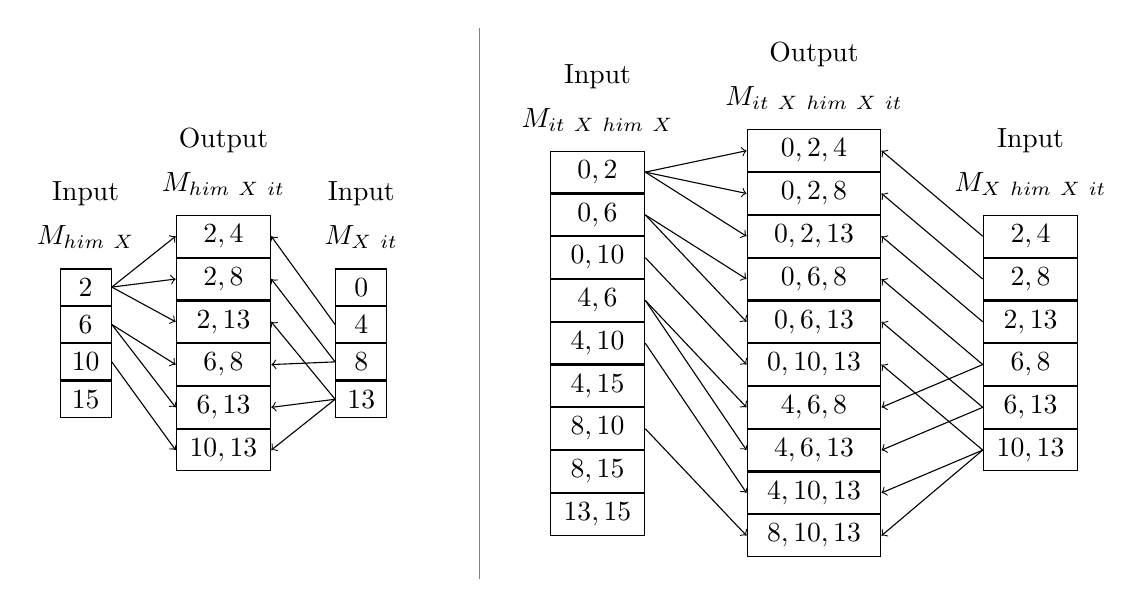
\begin{tikzpicture}[node distance=2.25cm]
	\matrix (him locations) [nodes={rectangle,draw,minimum width=6.5mm}]{
		\node (index 2)  {2}; \\
		\node (index 6)  {6}; \\
		\node (index 10) {10}; \\
		\node (index 15) {15}; \\
	};


	\matrix (him X it locations) [nodes={rectangle,draw,minimum width=12mm},right of=him locations,node distance=1.75cm]{
		\node (index 2 4)   {$2, 4$}; \\
		\node (index 2 8)   {$2, 8$}; \\
		\node (index 2 13)  {$2, 13$}; \\
		\node (index 6 8)   {$6, 8$}; \\
		\node (index 6 13)  {$6, 13$}; \\
		\node (index 10 13) {$10, 13$}; \\
	};


	\matrix (it locations) [nodes={rectangle,draw,minimum width=6.5mm},right of=him X it locations,node distance=1.75cm]{
		\node (index 0)  {0}; \\
		\node (index 4)  {4}; \\
		\node (index 8)  {8}; \\
		\node (index 13) {13}; \\
	};
	
	\node (him label) [anchor=south] at (him locations.north) {$M_{him~X}$};
	\node (pair label) [anchor=south] at (him X it locations.north) {$M_{him~X~it}$};
	\node (it label) [anchor=south] at (it locations.north) {$M_{X~it}$};
	\node [anchor=south] at (him label.north) {Input};
	\node [anchor=south] at (pair label.north) {Output};
	\node [anchor=south] at  (it label.north) {Input};

	\draw[->] (index 2.east) -- (index 2 4.west);
	\draw[->] (index 2.east) -- (index 2 8.west);
	\draw[->] (index 2.east) -- (index 2 13.west);
	\draw[->] (index 6.east) -- (index 6 8.west);
	\draw[->] (index 6.east) -- (index 6 13.west);
	\draw[->] (index 10.east) -- (index 10 13.west);

	\draw[->] (index 4.west) -- (index 2 4.east);
	\draw[->] (index 8.west) -- (index 2 8.east);
	\draw[->] (index 8.west) -- (index 6 8.east);
	\draw[->] (index 13.west) -- (index 2 13.east);
	\draw[->] (index 13.west) -- (index 6 13.east);
	\draw[->] (index 13.west) -- (index 10 13.east);

	\node (between)[right of=it locations,node distance=1.5cm] {};
	\draw[gray,thin] (between.center) -- +(0cm, 4cm);
	\draw[gray,thin] (between.center) -- +(0cm,-3cm);

	\matrix (it X him locations) [nodes={rectangle,draw,minimum width=12mm},right of=it locations,node distance=3cm]{
		\node (index 0 2)   {$0,2$}; \\
		\node (index 0 6)   {$0,6$}; \\
		\node (index 0 10)   {$0,10$}; \\
		\node (index 4 6)   {$4,6$}; \\
		\node (index 4 10)   {$4,10$}; \\
		\node (index 4 15)   {$4,15$}; \\
		\node (index 8 10)   {$8,10$}; \\
		\node (index 8 15)   {$8,15$}; \\
		\node (index 13 15)  {$13,15$}; \\
	};

	\matrix (it X him X it locations) [nodes={rectangle,draw,minimum width=17mm},right of=it X him locations,node distance=2.75cm]{
		\node (index 0 2 4)  {$0,2,4$}; \\
		\node (index 0 2 8)  {$0,2,8$}; \\
		\node (index 0 2 13)  {$0,2,13$}; \\
		\node (index 0 6 8)  {$0,6,8$}; \\
		\node (index 0 6 13)  {$0,6,13$}; \\
		\node (index 0 10 13)  {$0,10,13$}; \\
		\node (index 4 6 8)  {$4,6,8$}; \\
		\node (index 4 6 13)  {$4,6,13$}; \\
		\node (index 4 10 13)  {$4,10,13$}; \\
		\node (index 8 10 13)  {$8,10,13$}; \\
	};


	\matrix (him X it locations) [nodes={rectangle,draw,minimum width=12mm},right of=it X him X it locations,node distance=2.75cm]{
		\node (index 2 4)   {$2, 4$}; \\
		\node (index 2 8)   {$2, 8$}; \\
		\node (index 2 13)  {$2, 13$}; \\
		\node (index 6 8)   {$6, 8$}; \\
		\node (index 6 13)  {$6, 13$}; \\
		\node (index 10 13) {$10, 13$}; \\
	};

	\node (him label) [anchor=south] at (him X it locations.north) {$M_{X~him~X~it}$};
	\node (pair label) [anchor=south] at (it X him X it locations.north) {$M_{it~X~him~X~it}$};
	\node (it label) [anchor=south] at (it X him locations.north) {$M_{it~X~him~X}$};
	\node [anchor=south] at (him label.north) {Input};
	\node [anchor=south] at (pair label.north) {Output};
	\node [anchor=south] at  (it label.north) {Input};

	\draw[->] (index 0 2.east) -- (index 0 2 4.west);
	\draw[->] (index 0 2.east) -- (index 0 2 8.west);
	\draw[->] (index 0 2.east) -- (index 0 2 13.west);
	\draw[->] (index 0 6.east) -- (index 0 6 8.west);
	\draw[->] (index 0 6.east) -- (index 0 6 13.west);
	\draw[->] (index 0 10.east) -- (index 0 10 13.west);
	\draw[->] (index 4 6.east) --  (index 4 6 8.west);
	\draw[->] (index 4 6.east) --  (index 4 6 13.west);
	\draw[->] (index 4 10.east) -- (index 4 10 13.west);
	\draw[->] (index 8 10.east) -- (index 8 10 13.west);

	\draw[->] (index 2 4.west) -- (index 0 2 4.east);
	\draw[->] (index 2 8.west) -- (index 0 2 8.east);
	\draw[->] (index 2 13.west) -- (index 0 2 13.east);
	\draw[->] (index 6 8.west) --  (index 0 6 8.east);
	\draw[->] (index 6 13.west) -- (index 0 6 13.east);
	\draw[->] (index 6 8.west) --  (index 4 6 8.east);
	\draw[->] (index 6 13.west) -- (index 4 6 13.east);
	\draw[->] (index 10 13.west) -- (index 0 10 13.east);
	\draw[->] (index 10 13.west) -- (index 4 10 13.east);
	\draw[->] (index 10 13.west) -- (index 8 10 13.east);

\end{tikzpicture}






	\end{center}}
	\figpostamble
	\caption[\queryfunc\ examples.]{\queryfunc\ examples showing all input and output
	 	sets in sorted order and identifying the pair of input
		matchings that contribute to each output matching.}
	\label{fig:merge-example}
\end{figure}


\noindent Let's turn to the design of the \queryfunc\ algorithm that finds these partners.
First, consider a simple algorithm \intersectfunc\ on two sorted sets $L_1$ and $L_2$.
It computes sorted output set $L_{1 \cap 2}$ containing all
elements common to both $L_1$ and $L_2$ by iteratively comparing the
their topmost elements.  At each iteration, the lesser of the 
two elements is popped from its respective set and discarded.  If the elements
are equal, both are popped and a copy is appended to $L_{1 \cap 2}$.
The complexity of \intersectfunc\ is linear, $O(|L_1| + |L_2|)$.

We can implement \queryfunc\ using
roughly the same logic as \intersectfunc\ if 
$M_{a\alpha}$ and $M_{\alpha{}b}$ are sorted.
For the moment, we will simply assume sortedness.  Later, we will
show how this property is maintained.
The comparison operators that we have defined for partners will
stand in for the comparisons in \intersectfunc.
However, we still need to address a few subtleties.
An important difference between \queryfunc\ and \intersectfunc\
should be apparent from an inspection of example inputs and
outputs (Figure~\ref{fig:merge-example}).  It is possible 
that a matching from either input list partners with multiple
matchings from the other set.  We don't want to pop an item
from the set until we are certain that we have found all of
its partners.

\figpreamble
\begin{figure}
	\figfontsize{
	\begin{center}
		\begin{tikzpicture}[node distance=2.25cm]
	\matrix (him locations) [nodes={rectangle,draw,minimum width=6.5mm}]{
		\node (index 2)  {2}; \\
		\node [fill=lightgray](index 6)  {6}; \\
		\node (index 10) {10}; \\
		\node (index 15) {15}; \\
	};


	\matrix (him X it locations) [nodes={rectangle,draw,minimum width=12mm},right of=him locations,node distance=1.75cm]{
		\node (index 2 4)   {$2, 4$}; \\
		\node (index 2 8)   {$2, 8$}; \\
		\node (index 2 13)  {$2, 13$}; \\
		\node [fill=lightgray](index 6 8)   {$6, 8$}; \\
		\node [fill=lightgray](index 6 13)  {$6, 13$}; \\
		\node (index 10 13) {$10, 13$}; \\
	};


	\matrix (it locations) [nodes={rectangle,draw,minimum width=6.5mm},right of=him X it locations,node distance=1.75cm]{
		\node (index 0)  {0}; \\
		\node (index 4)  {4}; \\
		\node [fill=lightgray](index 8)  {8}; \\
		\node [fill=lightgray](index 13) {13}; \\
	};

	\draw[snake=brace,raise snake=1mm] (index 0.north east) -- (index 4.south east);
	\draw[snake=brace,raise snake=1mm] (index 8.north east) -- (index 13.south east);
%	\node [anchor=west,right=2mm] at (index 0.south east) {$(6) \ddot{>} q_{X~it}$};
%	\node [anchor=west,right=2mm] at (index 8.south east) {$(6) \ddot{=} q_{X~it}$};
	\node [anchor=west,right=2mm] at (index 0.south east) {$\ddot{>}$};
	\node (equal)[anchor=west,right=2mm] at (index 8.south east) {$\ddot{=}$};
	\node [anchor=north,below=4mm] at (equal.south) {$\ddot{<}$ is $\emptyset$};

	\node (him label) [anchor=south] at (him locations.north) {$M_{him~X}$};
	\node (pair label) [anchor=south] at (him X it locations.north) {$M_{him~X~it}$};
	\node (it label) [anchor=south] at (it locations.north) {$M_{X~it}$};
	\node [anchor=south] at (him label.north) {Input};
	\node [anchor=south] at (pair label.north) {Output};
	\node [anchor=south] at  (it label.north) {Input};

	\fill[lightgray] 
		(index 6.south east) --
		(index 6.north east) --
		(index 6 8.north west) --
		(index 6 13.south west) -- cycle;

	\fill[lightgray] 
		(index 6 13.south east) --
		(index 6 8.north east) --
		(index 8.north west) --
		(index 13.south west) -- cycle;
		

	\draw[->] (index 2.east) -- (index 2 4.west);
	\draw[->] (index 2.east) -- (index 2 8.west);
	\draw[->] (index 2.east) -- (index 2 13.west);
	\draw[->] (index 6.east) -- (index 6 8.west);
	\draw[->] (index 6.east) -- (index 6 13.west);
	\draw[->] (index 10.east) -- (index 10 13.west);

	\draw[->] (index 4.west) -- (index 2 4.east);
	\draw[->] (index 8.west) -- (index 2 8.east);
	\draw[->] (index 8.west) -- (index 6 8.east);
	\draw[->] (index 13.west) -- (index 2 13.east);
	\draw[->] (index 13.west) -- (index 6 13.east);
	\draw[->] (index 13.west) -- (index 10 13.east);


	\node (between)[right of=it locations,node distance=1.5cm] {};
	\draw[gray,thin] (between.center) -- +(0cm, 4cm);
	\draw[gray,thin] (between.center) -- +(0cm,-3cm);

	\matrix (it X him locations) [nodes={rectangle,draw,minimum width=12mm},right of=it locations,node distance=3cm]{
		\node (index 0 2)   {$0,2$}; \\
		\node (index 0 6)   {$0,6$}; \\
		\node (index 0 10)   {$0,10$}; \\
		\node [fill=lightgray](index 4 6)   {$4,6$}; \\
		\node (index 4 10)   {$4,10$}; \\
		\node (index 4 15)   {$4,15$}; \\
		\node (index 8 10)   {$8,10$}; \\
		\node (index 8 15)   {$8,15$}; \\
		\node (index 13 15)  {$13,15$}; \\
	};

	\matrix (it X him X it locations) [nodes={rectangle,draw,minimum width=17mm},right of=it X him locations,node distance=2.75cm]{
		\node (index 0 2 4)  {$0,2,4$}; \\
		\node (index 0 2 8)  {$0,2,8$}; \\
		\node (index 0 2 13)  {$0,2,13$}; \\
		\node (index 0 6 8)  {$0,6,8$}; \\
		\node (index 0 6 13)  {$0,6,13$}; \\
		\node (index 0 10 13)  {$0,10,13$}; \\
		\node [fill=lightgray](index 4 6 8)  {$4,6,8$}; \\
		\node [fill=lightgray](index 4 6 13)  {$4,6,13$}; \\
		\node (index 4 10 13)  {$4,10,13$}; \\
		\node (index 8 10 13)  {$8,10,13$}; \\
	};


	\matrix (him X it locations) [nodes={rectangle,draw,minimum width=12mm},right of=it X him X it locations,node distance=2.75cm]{
		\node (index 2 4)   {$2, 4$}; \\
		\node (index 2 8)   {$2, 8$}; \\
		\node (index 2 13)  {$2, 13$}; \\
		\node [fill=lightgray](index 6 8)   {$6, 8$}; \\
		\node [fill=lightgray](index 6 13)  {$6, 13$}; \\
		\node (index 10 13) {$10, 13$}; \\
	};

	\draw[snake=brace,raise snake=1mm] (index 2 4.north east) -- (index 2 13.south east);
	\draw[snake=brace,raise snake=1mm] (index 6 8.north east) -- (index 6 13.south east);
	\draw[snake=brace,raise snake=1mm] (index 10 13.north east) -- (index 10 13.south east);
%	\node [anchor=west,right=2mm] at (index 2 8.east) {$(4,6) \ddot{>} q_{X~him~X~it}$};
%	\node [anchor=west,right=2mm] at (index 6 8.south east) {$(4,6) \ddot{=} q_{X~him~X~it}$};
%	\node [anchor=west,right=2mm] at (index 10 13.east) {$(4,6) \ddot{<} q_{X~him~X~it}$};
	\node [anchor=west,right=2mm] at (index 2 8.east) {$\ddot{>}$};
	\node [anchor=west,right=2mm] at (index 6 8.south east) {$\ddot{=}$};
	\node [anchor=west,right=2mm] at (index 10 13.east) {$\ddot{<}$};


	\node (him label) [anchor=south] at (him X it locations.north) {$M_{X~him~X~it}$};
	\node (pair label) [anchor=south] at (it X him X it locations.north) {$M_{it~X~him~X~it}$};
	\node (it label) [anchor=south] at (it X him locations.north) {$M_{it~X~him~X}$};
	\node [anchor=south] at (him label.north) {Input};
	\node [anchor=south] at (pair label.north) {Output};
	\node [anchor=south] at  (it label.north) {Input};

	\fill[lightgray] 
		(index 4 6.south east) --
		(index 4 6.north east) --
		(index 4 6 8.north west) --
		(index 4 6 13.south west) -- cycle;

	\fill[lightgray] 
		(index 4 6 13.south east) --
		(index 4 6 8.north east) --
		(index 6 8.north west) --
		(index 6 13.south west) -- cycle;


	\draw[->] (index 0 2.east) -- (index 0 2 4.west);
	\draw[->] (index 0 2.east) -- (index 0 2 8.west);
	\draw[->] (index 0 2.east) -- (index 0 2 13.west);
	\draw[->] (index 0 6.east) -- (index 0 6 8.west);
	\draw[->] (index 0 6.east) -- (index 0 6 13.west);
	\draw[->] (index 0 10.east) -- (index 0 10 13.west);
	\draw[->] (index 4 6.east) --  (index 4 6 8.west);
	\draw[->] (index 4 6.east) --  (index 4 6 13.west);
	\draw[->] (index 4 10.east) -- (index 4 10 13.west);
	\draw[->] (index 8 10.east) -- (index 8 10 13.west);

	\draw[->] (index 2 4.west) -- (index 0 2 4.east);
	\draw[->] (index 2 8.west) -- (index 0 2 8.east);
	\draw[->] (index 2 13.west) -- (index 0 2 13.east);
	\draw[->] (index 6 8.west) --  (index 0 6 8.east);
	\draw[->] (index 6 13.west) -- (index 0 6 13.east);
	\draw[->] (index 6 8.west) --  (index 4 6 8.east);
	\draw[->] (index 6 13.west) -- (index 4 6 13.east);
	\draw[->] (index 10 13.west) -- (index 0 10 13.east);
	\draw[->] (index 10 13.west) -- (index 4 10 13.east);
	\draw[->] (index 10 13.west) -- (index 8 10 13.east);

\end{tikzpicture}

	\end{center}}
	\figpostamble
	\caption{Examples showing the division of $M_{\alpha{}b}$
		into regions by $m_{a\alpha} \in M_{a\alpha}$.}
	\label{fig:prefix-region}
\end{figure}

Let's first consider a matching $m_{a\alpha}$ of prefix
pattern $a\alpha$.  Let $m_\alpha = s(m_{a\alpha})$.
Any partner $m_{\alpha{}b}$ must satisfy the constraint
$p(m_{\alpha{}b}) = m_\alpha$.  From the definition of
the prefix matching, we see that if $\alpha = \beta{}c$,
then the only valid value for $m_{\alpha{}b}$ is in 
fact $m_\alpha$.  If $\alpha = \beta{}X$, then $m_\alpha$
completely determines all elements of $m_{\alpha{}b}$ except
for the final one, $m_{\alpha{}b,K_{\alpha{}b}}$.  In either case,
since $M_{\alpha{}b}$ is sorted, all matchings of $\alpha{}b$
meeting the constraint must occur in the same (possibly empty) 
contiguous region of $M_{\alpha{}b}$.  Sortedness further
guarantees that for all elements $m_{\alpha{}b} \in M_{\alpha{}b}$
subsequent to this region,
$m_{a\alpha} \ddot{<} m_{\alpha{}b}$ by definition of the
comparison operators.  It likewise guarantees that for 
all elements $m_{\alpha{}b} \in M_{\alpha{}b}$ prior to this region,
$m_{a\alpha} \ddot{>} m_{\alpha{}b}$.  Therefore, matching
$m_{a\alpha}$ divides $M_{\alpha{}b}$ into three distinct
regions, any of which may be empty (Figure~\ref{fig:prefix-region}).
This means that we can pop
$m_{a\alpha}$ when we encounter the first element 
$m_{\alpha{}b}$ such that $m_{a\alpha} \ddot{<} m_{\alpha{}b}$
or when we reach the end of the set.

\figpreamble
\begin{figure}
	\figfontsize{
	\begin{center}
		\begin{tikzpicture}[node distance=2.25cm]

	\matrix (it X him locations) [nodes={rectangle,draw,minimum width=12mm}]{
		\node (index 0 2)   {$0,2$}; \\
		\node [fill=lightgray](index 0 6)   {$0,6$}; \\
		\node (index 0 10)   {$0,10$}; \\
		\node [fill=lightgray](index 4 6)   {$4,6$}; \\
		\node (index 4 10)   {$4,10$}; \\
		\node (index 4 15)   {$4,15$}; \\
		\node (index 8 10)   {$8,10$}; \\
		\node (index 8 15)   {$8,15$}; \\
		\node (index 13 15)  {$13,15$}; \\
	};

	\node [anchor=east] at (index 0 2.west) {$\ddot{<}$};
	\node [anchor=east] at (index 0 6.west) {$\ddot{=}$};
	\node [anchor=east] at (index 0 10.west) {$\ddot{>}$};
	\node [anchor=east] at (index 4 6.west) {$\ddot{=}$};
	\node [anchor=east] at (index 4 10.west) {$\ddot{>}$};
	\node [anchor=east] at (index 4 15.west) {$\ddot{>}$};
	\node [anchor=east] at (index 8 10.west) {$\ddot{>}$};
	\node [anchor=east] at (index 8 15.west) {$\ddot{>}$};
	\node [anchor=east] at (index 13 15.west) {$\ddot{>}$};

	\matrix (it X him X it locations) [nodes={rectangle,draw,minimum width=17mm},right of=it X him locations,node distance=2.5cm]{
		\node (index 0 2 4)  {$0,2,4$}; \\
		\node (index 0 2 8)  {$0,2,8$}; \\
		\node (index 0 2 13)  {$0,2,13$}; \\
		\node [fill=lightgray](index 0 6 8)  {$0,6,8$}; \\
		\node (index 0 6 13)  {$0,6,13$}; \\
		\node (index 0 10 13)  {$0,10,13$}; \\
		\node [fill=lightgray](index 4 6 8)  {$4,6,8$}; \\
		\node (index 4 6 13)  {$4,6,13$}; \\
		\node (index 4 10 13)  {$4,10,13$}; \\
		\node (index 8 10 13)  {$8,10,13$}; \\
	};


	\matrix (him X it locations) [nodes={rectangle,draw,minimum width=12mm},right of=it X him X it locations,node distance=2.5cm]{
		\node (index 2 4)   {$2, 4$}; \\
		\node (index 2 8)   {$2, 8$}; \\
		\node (index 2 13)  {$2, 13$}; \\
		\node [fill=lightgray](index 6 8)   {$6, 8$}; \\
		\node (index 6 13)  {$6, 13$}; \\
		\node (index 10 13) {$10, 13$}; \\
	};

	\fill[lightgray]
		(index 0 6.south east) --
		(index 0 6.north east) --
		(index 0 6 8.north west) --
		(index 0 6 8.south west) --cycle;

	\fill[lightgray]
		(index 4 6.south east) --
		(index 4 6.north east) --
		(index 4 6 8.north west) --
		(index 4 6 8.south west) --cycle;

	\fill[lightgray]
		(index 0 6 8.south east) --
		(index 0 6 8.north east) --
		(index 6 8.north west) --
		(index 6 8.south west) --cycle;

	\fill[lightgray]
		(index 4 6 8.south east) --
		(index 4 6 8.north east) --
		(index 6 8.north west) --
		(index 6 8.south west) --cycle;



	\node (him label) [anchor=south] at (him X it locations.north) {$M_{him~X~it~X}$};
	\node (pair label) [anchor=south] at (it X him X it locations.north) {$M_{it~X~him~X~it}$};
	\node (it label) [anchor=south] at (it X him locations.north) {$M_{X~it~X~him}$};
	\node [anchor=south] at (him label.north) {Input};
	\node [anchor=south] at (pair label.north) {Output};
	\node [anchor=south] at  (it label.north) {Input};

	\draw[->] (index 0 2.east) -- (index 0 2 4.west);
	\draw[->] (index 0 2.east) -- (index 0 2 8.west);
	\draw[->] (index 0 2.east) -- (index 0 2 13.west);
	\draw[->] (index 0 6.east) -- (index 0 6 8.west);
	\draw[->] (index 0 6.east) -- (index 0 6 13.west);
	\draw[->] (index 0 10.east) -- (index 0 10 13.west);
	\draw[->] (index 4 6.east) --  (index 4 6 8.west);
	\draw[->] (index 4 6.east) --  (index 4 6 13.west);
	\draw[->] (index 4 10.east) -- (index 4 10 13.west);
	\draw[->] (index 8 10.east) -- (index 8 10 13.west);

	\draw[->] (index 2 4.west) -- (index 0 2 4.east);
	\draw[->] (index 2 8.west) -- (index 0 2 8.east);
	\draw[->] (index 2 13.west) -- (index 0 2 13.east);
	\draw[->] (index 6 8.west) --  (index 0 6 8.east);
	\draw[->] (index 6 13.west) -- (index 0 6 13.east);
	\draw[->] (index 6 8.west) --  (index 4 6 8.east);
	\draw[->] (index 6 13.west) -- (index 4 6 13.east);
	\draw[->] (index 10 13.west) -- (index 0 10 13.east);
	\draw[->] (index 10 13.west) -- (index 4 10 13.east);
	\draw[->] (index 10 13.west) -- (index 8 10 13.east);


	\node (separator) [right of=him X it locations,node distance=1.25cm] {}; 
	\draw[gray,thin] (separator.center) -- +(0cm,4cm);
	\draw[gray,thin] (separator.center) -- +(0cm,-3cm);

	\matrix (it X him locations) [nodes={rectangle,draw,minimum width=12mm},right of=him X it locations,node distance=3cm]{
		\node (index 0 2)   {$\colorbox{lightgray}{0},2$}; \\
		\node [fill=lightgray](index 0 6)   {$\colorbox{lightgray}{0},6$}; \\
		\node (index 0 10)   {$\colorbox{lightgray}{0},10$}; \\
		\node [fill=lightgray](index 4 6)   {$\colorbox{lightgray}{4},6$}; \\
		\node (index 4 10)   {$\colorbox{lightgray}{4},10$}; \\
		\node (index 4 15)   {$\colorbox{lightgray}{4},15$}; \\
		\node (index 8 10)   {$8,10$}; \\
		\node (index 8 15)   {$8,15$}; \\
		\node (index 13 15)  {$13,15$}; \\
	};

	\draw[snake=brace,raise snake=1mm] (index 4 15.south west) -- (index 0 2.north west);
	\draw[snake=brace,raise snake=1mm] (index 13 15.south west) -- (index 8 10.north west);
	\node[anchor=east,left=2mm,text width=4mm] at (index 0 10.south west) {$\ddot{<}$, $\ddot{=}$, or $\ddot{>}$};
	\node[anchor=east,left=2mm] at (index 8 15.west) {$\ddot{>}$};

	\matrix (it X him X it locations) [nodes={rectangle,draw,minimum width=17mm},right of=it X him locations,node distance=2.5cm]{
		\node (index 0 2 4)  {$0,2,4$}; \\
		\node (index 0 2 8)  {$0,2,8$}; \\
		\node (index 0 2 13)  {$0,2,13$}; \\
		\node [fill=lightgray](index 0 6 8)  {$0,6,8$}; \\
		\node (index 0 6 13)  {$0,6,13$}; \\
		\node (index 0 10 13)  {$0,10,13$}; \\
		\node [fill=lightgray](index 4 6 8)  {$4,6,8$}; \\
		\node (index 4 6 13)  {$4,6,13$}; \\
		\node (index 4 10 13)  {$4,10,13$}; \\
		\node (index 8 10 13)  {$8,10,13$}; \\
	};


	\matrix (him X it locations) [nodes={rectangle,draw,minimum width=12mm},right of=it X him X it locations,node distance=2.5cm]{
		\node (index 2 4)   {$2, 4$}; \\
		\node (index 2 8)   {$2, 8$}; \\
		\node (index 2 13)  {$2, 13$}; \\
		\node [fill=lightgray](index 6 8)   {$6, 8$}; \\
		\node (index 6 13)  {$6, 13$}; \\
		\node (index 10 13) {$10, 13$}; \\
	};

	\fill[lightgray]
		(index 0 6.south east) --
		(index 0 6.north east) --
		(index 0 6 8.north west) --
		(index 0 6 8.south west) --cycle;

	\fill[lightgray]
		(index 4 6.south east) --
		(index 4 6.north east) --
		(index 4 6 8.north west) --
		(index 4 6 8.south west) --cycle;

	\fill[lightgray]
		(index 0 6 8.south east) --
		(index 0 6 8.north east) --
		(index 6 8.north west) --
		(index 6 8.south west) --cycle;

	\fill[lightgray]
		(index 4 6 8.south east) --
		(index 4 6 8.north east) --
		(index 6 8.north west) --
		(index 6 8.south west) --cycle;

	\node (him label) [anchor=south] at (him X it locations.north) {$M_{X~him~X~it}$};
	\node (pair label) [anchor=south] at (it X him X it locations.north) {$M_{it~X~him~X~it}$};
	\node (it label) [anchor=south] at (it X him locations.north) {$M_{it~X~him~X}$};
	\node [anchor=south] at (him label.north) {Input};
	\node [anchor=south] at (pair label.north) {Output};
	\node [anchor=south] at  (it label.north) {Input};

	\draw[->] (index 0 2.east) -- (index 0 2 4.west);
	\draw[->] (index 0 2.east) -- (index 0 2 8.west);
	\draw[->] (index 0 2.east) -- (index 0 2 13.west);
	\draw[->] (index 0 6.east) -- (index 0 6 8.west);
	\draw[->] (index 0 6.east) -- (index 0 6 13.west);
	\draw[->] (index 0 10.east) -- (index 0 10 13.west);
	\draw[->] (index 4 6.east) --  (index 4 6 8.west);
	\draw[->] (index 4 6.east) --  (index 4 6 13.west);
	\draw[->] (index 4 10.east) -- (index 4 10 13.west);
	\draw[->] (index 8 10.east) -- (index 8 10 13.west);

	\draw[->] (index 2 4.west) -- (index 0 2 4.east);
	\draw[->] (index 2 8.west) -- (index 0 2 8.east);
	\draw[->] (index 2 13.west) -- (index 0 2 13.east);
	\draw[->] (index 6 8.west) --  (index 0 6 8.east);
	\draw[->] (index 6 13.west) -- (index 0 6 13.east);
	\draw[->] (index 6 8.west) --  (index 4 6 8.east);
	\draw[->] (index 6 13.west) -- (index 4 6 13.east);
	\draw[->] (index 10 13.west) -- (index 0 10 13.east);
	\draw[->] (index 10 13.west) -- (index 4 10 13.east);
	\draw[->] (index 10 13.west) -- (index 8 10 13.east);

\end{tikzpicture}

	\end{center}}
	\figpostamble
	\caption[xample showing the relationships of $m_{a\alpha} \in M_{a\alpha}$
		to an element $m_{\alpha{}b}$.]{Example showing the relationships of $m_{a\alpha} \in M_{a\alpha}$ to an element $m_{\alpha{}b}$, and the subsequent delineation of
		$M_{a\alpha}$ into regions by $m_{\alpha{}b}$.}
	\label{fig:suffix-region}
\end{figure}

Now let's consider a matching $m_{\alpha{}b}$ of suffix
pattern $\alpha{}b$.  Let $m_\alpha = p(m_{\alpha{}b})$.
Any partner $m_{a\alpha}$ must satisfy the constraint
$s(m_{a\alpha}) = m_\alpha$.  From the definition of
the suffix matching, we see that if $\alpha = c\beta$,
then there is only one valid value for $m_{a\alpha}$.  In
this case, sortedness ensures that $m_{\alpha{}b}$
divides $M_{a\alpha}$ into three regions, just as we
saw for the prefix matchings.  Matters are different
if $\alpha = X\beta$.  In this case, $m_\alpha$
completely determines all elements of $m_{a\alpha}$
except for the first one, $m_{a\alpha,1}$.  This element
could take several values.  Furthermore, each of these values 
can be the first element of several matchings.  Only one of
these matching will meet our constraint, and thus
the rest won't be partners with $m_{\alpha{}b}$.  As a consequence,
it is possible for partners of $m_{\alpha{}b}$ to be 
interspersed with non-partners (Figure~\ref{fig:suffix-region}).
However, our definitions ensure that there is a contiguous 
range of possible values for $m_{\alpha{}b,1}$.
Sortedness ensures that the set of all matchings 
$m_{a\alpha} \in M_{a\alpha}$ for which $m_{\alpha{}b,1}$ is in this
range must occur in a contiguous region of $M_{a\alpha}$.
Furthermore, our definitions ensure that for any 
value $i$, if $m_{a\alpha} \ddot{>} m_{\alpha{}b}$ for the first occurrence
of a matching $m_{a\alpha}$ such $m_{ab\alpha,1} = i$,
then for all subsequent matchings $m_{a\alpha} \in M_{a\alpha}$,
$m_{a\alpha} \ddot{>} m_{\alpha{}b}$.  An analogous case
occurs for matchings $m_{a\alpha} \in M_{a\alpha}$ such that
$m_{a\alpha} \ddot{<} m_{\alpha{}b}$.  Therefore, $m_{\alpha{}b}$
divide $M_{a\alpha}$ into three regions, each of which may
possibly be empty.  However, it is possible for values in
the central region to have any relationship with $m_{\alpha{}b}$,
and therefore we must check all of them.  We can safely
pop $m_{\alpha{}b}$ when we encounter a matching
$m_{a\alpha}$ such that $m_{a\alpha} \ddot{>} m_{\alpha{}b}$ and
whose first element $m_{a\alpha,1}$ has not been seen before.

\algorithm{The basic \queryfunc\ algorithm}{
	\label{alg:query-intersect}
	\noindent {\bf Function} {\sc Query\_Intersect}

\noindent {\bf Input:} sorted prefix matchings $M_{a\alpha}$ and sorted suffix matchings $M_{\alpha{}b}$
\begin{algorithmic}[1]

	\State $M_{a\alpha{}b} \leftarrow \emptyset$
	\State $I \leftarrow |M_{a\alpha}|$
	\State $J \leftarrow |M_{\alpha{}b}|$
	\State $j \leftarrow 0$
	\State $m_1 \leftarrow -1$
	\For {$i$ from $0$ to $I$}
		\State $m_{a\alpha} \leftarrow M_{a\alpha}[i]$
		\State $m_{\alpha{}b} \leftarrow M_{\alpha{}b}[j]$
		\If {$m_{a\alpha,1} \neq m_1$}
			\While {$m_{a\alpha} \ddot{>} m_{\alpha{}b}$ and $j < J$}
				\State $j \leftarrow j + 1$
				\State $m_{\alpha{}b} \leftarrow M_{\alpha{}b}[j]$
			\EndWhile
			\If {$m_{a\alpha} \ddot{>} m_{\alpha{}b}$ and $j = J$}
				\State Break
			\EndIf
		\EndIf
		\State $k \leftarrow j$
		\While {not $m_{a\alpha} \ddot{<} m_{\alpha{}b}$}
			\If {$m_{a\alpha} \ddot{=} m_{\alpha{}b}$}
				\State Append $m_{a\alpha} \bowtie m_{\alpha{}b}$ to $M_{a\alpha{}b}$
			\EndIf
			\If {$k = J$}
				\State Break
			\Else
				\State $k \leftarrow k + 1$
				\State $m_{\alpha{}b} \leftarrow M_{\alpha{}b}[k]$
			\EndIf
		\EndWhile
	\EndFor
	\State \Return {$M_{a\alpha{}b}$}
\end{algorithmic}

}


The full \queryfunc\ algorithm (Listing~\ref{alg:query-intersect}) is non-destructive -- we
advance a pointer rather than popping matchings from each set.  Its operation is
similar to \intersectfunc, though we take a different approach to popping matchings
from the stack.  For each matching $m_{a\alpha} \in M_{a\alpha}$, we scan 
downwards from the current top of $M_{\alpha{}b}$, joining $m_{a\alpha}$ with any
partners as we find them, until we encounter $m_{\alpha{}b}$ such that
$m_{a\alpha} \ddot{<} m_{\alpha{}b}$.  We then pop $m_{a\alpha}$.  Elements
$m_{\alpha{}b} \in M_{\alpha{}b}$ are popped whenever we uncover a new
top matching $m_{a\alpha} \in M_{a\alpha}$ such that 
$m_{a\alpha} \ddot{>} m_{\alpha{}b}$ and whose first element $m_{a\alpha,1}$
has not been seen before.  

The upper bound complexity of \queryfunc\ is $O(|M_{a\alpha}| \times |M_{\alpha{}b}|)$.
However, most matchings can be popped from their respective sets after a single
comparison, so the average case complexity is closer to 
$O(|M_{a\alpha}| + |M_{\alpha{}b}|)$.  Both upper bound and average complexity are
identical to that of the baseline algorithm.  As we've seen, though, our
enumeration algorithm enables us to call it much less frequently using
smaller input sets than in the baseline.

We assume that $M_{a\alpha}$ is
sorted, and we process its matchings in order.  Furthermore, for any
$m_{a\alpha} \in M_{a\alpha}$, recall that its partners can only differ
on their last element, and that these are encountered in sorted order.
Therefore, the output of \queryfunc\ is sorted.  This means that
if we call \queryfunc\ using input sets that resulted from a previous
invocation of \queryfunc, they will already be sorted.
We must still ensure sortedness in the base case, which occurs when 
either prefix $a\alpha$ or suffix $\alpha{}b$ contains a single
contiguous pattern.  In this case, the set $M_{a\alpha}$ or
$M_{\alpha{}b}$ is the result of a search in the suffix array.
As we saw earlier, this set is not returned in sorted
order.  To solve this, we explicitly sort the occurrences by inserting
them into a stratified tree \citep{emde-boas:1977:mst} and
reading the sorted sequence from the tree.  Sort
time is $O(|M_\alpha| \log\log |T|)$ for a pattern $\alpha$.
This is superlinear, but we need to sort only
once, since we cache the result at the corresponding
prefix tree node.  Since we expect to query the text for many patterns containing this
subpattern, the cost is amortized over all computations.
Overall, this means that ensuring sortedness
adds computational expense to our algorithm.  
This will be counterbalanced by additional strategies that exploit
sortedness, introduced in the next sections.
